% !TEX root = ../gnss_interference_resistant_thesis.tex
\documentclass[../gnss_interference_resistant_thesis.tex]{subfiles}

\begin{document}

\section{Trigdžiams atspari sistema}

\subsection{HackRF One SDR imutvas/siustuvas}

HackRF One yra SDR imtuvas, kuris sugeba siųsti/priimti signalus ruože nuo
$1\ \mathrm{MHz}$ iki $6\ \mathrm{GHz}$ \cite{hackrf_one}.
HackRF imtuvas turi 8 bitų ADC, veikiantį iki $20\ \mathrm{MHz}$.
Imtuvo brėžiniai ir apartinė įranga yra atviro kodo, todėl visi
reikalingi pakeitimai gali būti nesunkiai įgyvendinti \cite{hackrf_github}.

\begin{figure}[h]
    \begin{centering}
    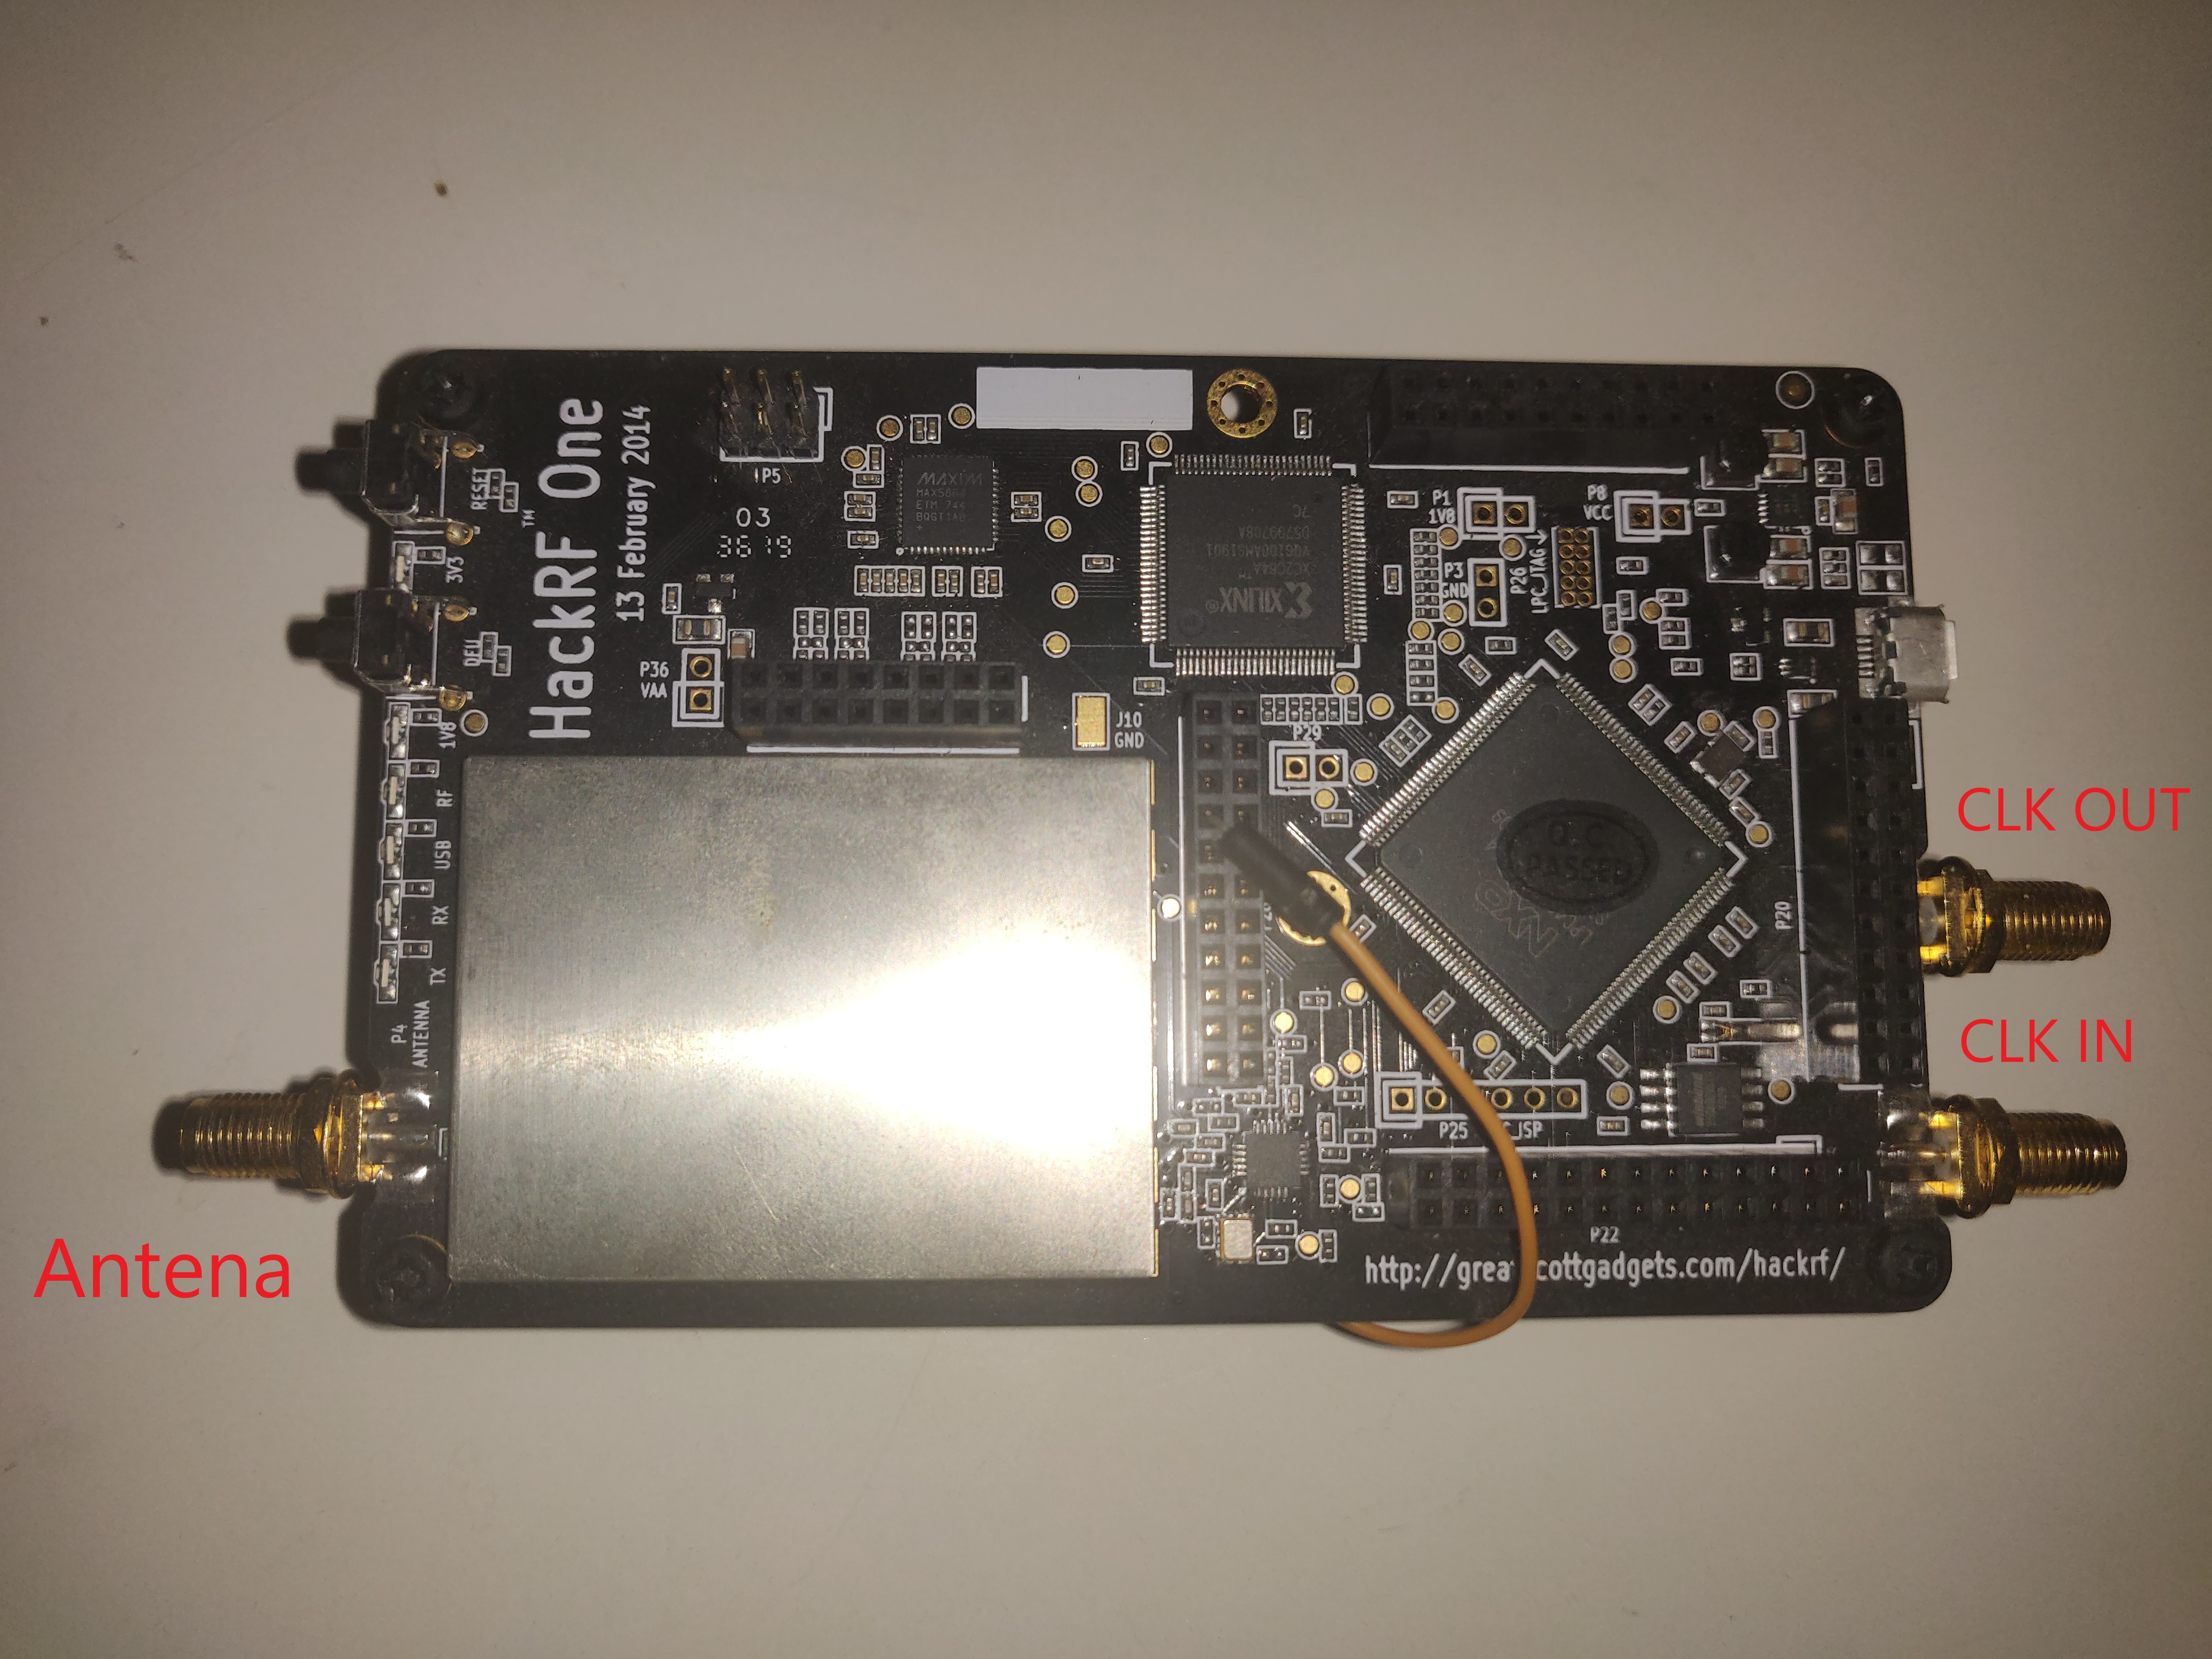
\includegraphics[scale=0.1]{drawings/hackrf_img}
    \par\end{centering}
    \protect\caption{\label{fig:hackrf_img}HackRF One nuotrauka su pažymėtais įėjimais ir išėjimais.}
\end{figure}

Norint atlikti spindulio formavimą, reikia tiek SDR imtuvų, kiek masyve
turėsime antenų. Kad būtų įmanoma atlikti spindulio formavimą, reikia laiko, dažnio ir fazės
sinchronizacijos tarp visų SDR imtuvų.
Dažnio sinchronizaciją pasiekti yra lengviausia, vieno imtuvo CLK OUT sujungiamas su
kitų imtuvų CLK IN, taip gaunama dažnio sinchronizacija, kadangi
visi imtuvai generuojasi taktinius dažnius iš to pačio šaltinio.

Laiko sincronizaciją pasiekti yra sudėtingiau. Prieš pradedant duomenų nuskaitymą,
kompiuterio operacinė sistema (OS), išssiunčia nuskaitymo pradžios komandą.
Kadangi OS sistema yra nenuspėjama, atsiranda tam tikri uždelsimai, tarp
visų nuskaitymo komandų. Kadangi imtuvai pradeda skaityti skirtingu metu,
nebeįmanoma sulyginti IQ taškų gautų kompiuteryje. Vienas iš galimų sprendimų
yra susinchronizuoti visų imtuvų nuskaitymo pradžia pasitelkus signalu,
kuris perduodamas ne per USB, tačiau tiesiogiai tarp imtuvų.
Toks metodas buvo ištyrinėtas ir nustatytą kad pasiekama sinchronizaciją
gerenė negu 1 nuskaitymo taškas \cite{hackrf_sync}.

\begin{figure}[h]
    \begin{centering}
    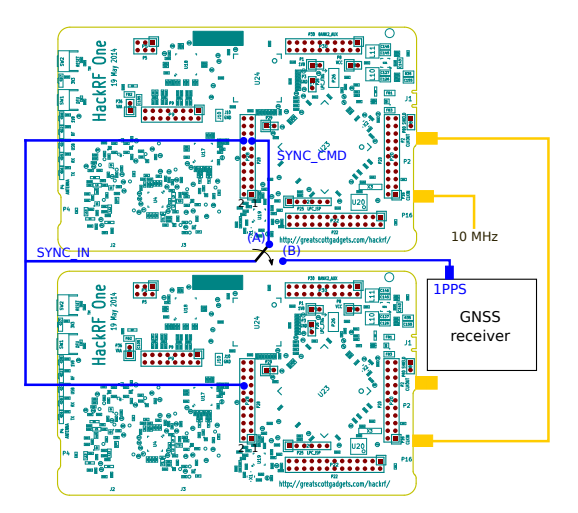
\includegraphics[scale=0.8]{drawings/hackrf_sync}
    \par\end{centering}
    \protect\caption{\label{fig:hackrf_sync}HackRF imtuvų sinchronizacijos schema \cite{hackrf_sync}.}
\end{figure}

Vienas iš imtuvų yra pasirenkamas kai valdantysis, kuris generuoja SYNC CMD signalą,
kiti kaip valdomieji, kurie laukia SYNC IN signalo. Kompiuteris
išssiunčia komandą į visus imtuvus, kad lauktų signalo iš vieno iš imtuvų,
valdančiajam imtuvui sugeneravus pradžios signalą, visi imtuvai vienu metu pradeda
nuskaitymą ir duomenų siuntimą į kompiuterį.

Fazinės kalibracijos įsijungimo metu pasiekti neįmanoma. Kadangi įsijungimo metu yra
paleidinėjami dažnio daugintuvai (PLL), jų pradinė fazė yr atsitiktinė.
Norint turėti vienodas fazes, reikia naudoti tą patį PLL šaltinį visiems
dažnių maišituvams. HackRF tokios galimybės neturi be didelių pakeitimų.
Kai SDR yra iniazilizuotas, jo fazė yra pakankamai stabili, kad būtų galima
vykdyti spindulio formavimą.
Tam kad iššisaiškinti imtuvų fazę, po kiekieno įjungimo reikia atlikti kalibraciją.
Į visų imtuvų iėjimą, paduodamas pastovus signalas, kompiuteryje yra išsaugomas
fazinis poslinkis tarp imptuvų. Baigus kalibraciją galima pradėti spindulio
formavimo operacijas.



\end{document}
